\begin{GreyBox}
    \vskip-1cm
    \begin{block}{\GHead{Results}} 
        \begin{center}
            \vspace{7mm}
            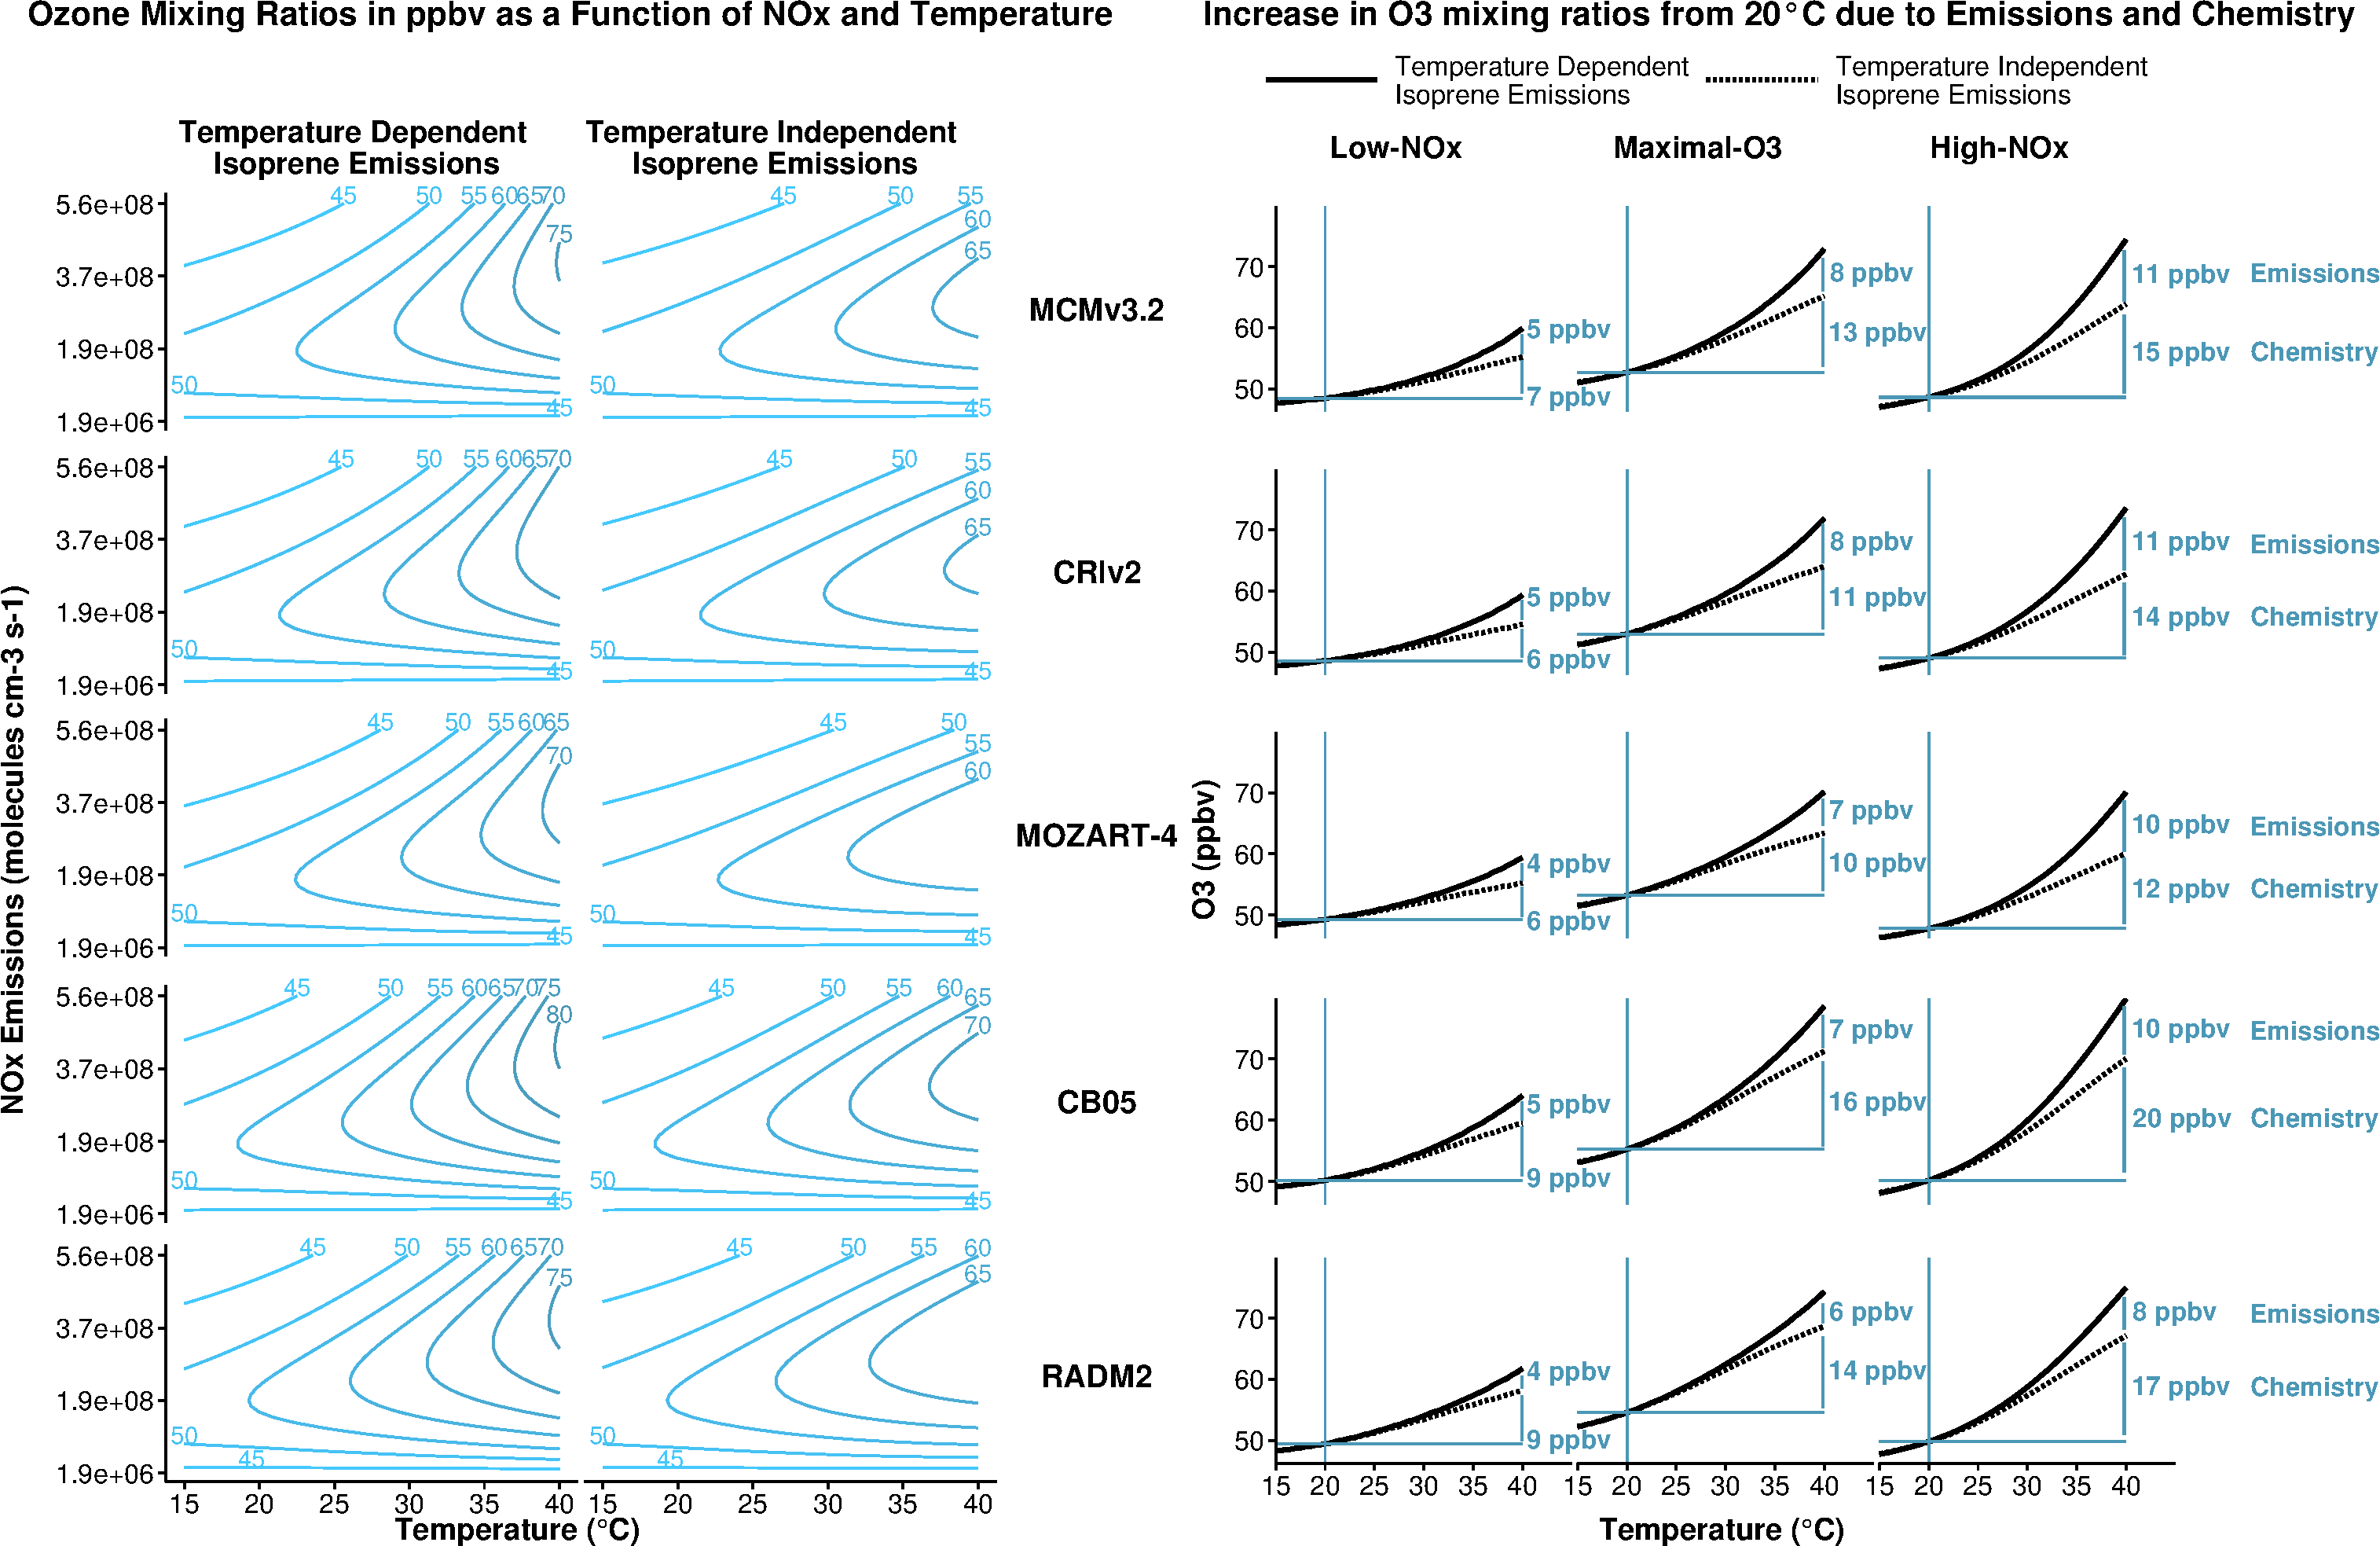
\includegraphics[width = \textwidth]{Plotting/results}
        \end{center}
        \begin{columns}[t]
            \column{0.45\textwidth}
                \begin{flushleft}
                    \begin{WhiteBox}
                        \begin{itemize} \vspace{8mm}
                            \item High-\ce{NO_x} and temperature-dependent isoprene $\Rightarrow$ highest ozone levels. \vspace{13mm}
                            \item Low-\ce{NO_x} conditions has lowest ozone levels. \vspace{13mm}
                            \item Ozone levels vary non-linearly with \ce{NO_x} and temperature in each chemical mechanism. \vspace{13mm}
                            \item RADM2 and CB05 produce most ozone regardless of isoprene source. %\vspace{13mm}
                        \end{itemize}
                    \end{WhiteBox}
                \end{flushleft}
            \column{0.45\textwidth}
                \begin{flushright}
                    \begin{WhiteBox} \vspace{8mm}
                        \begin{itemize}
                            \item Faster reaction rates cause larger increase in ozone than higher isoprene emissions. \vspace{13mm}
                            \item High-\ce{NO_x} conditions has largest increases in ozone from chemistry and emissions. \vspace{13mm}
                            \item Increased isoprene emissions in CB05 and RADM2 produces less ozone than other chemical mechanisms. %\vspace{13mm} 
                        \end{itemize}
                    \end{WhiteBox}
                \end{flushright}
        \end{columns}
    \end{block}
\end{GreyBox}
